\section{First Dialog}

After the application was started a dialog for opening/creating a databases is shown. 

\begin{figure}[H]
  \hspace*{-2cm}
    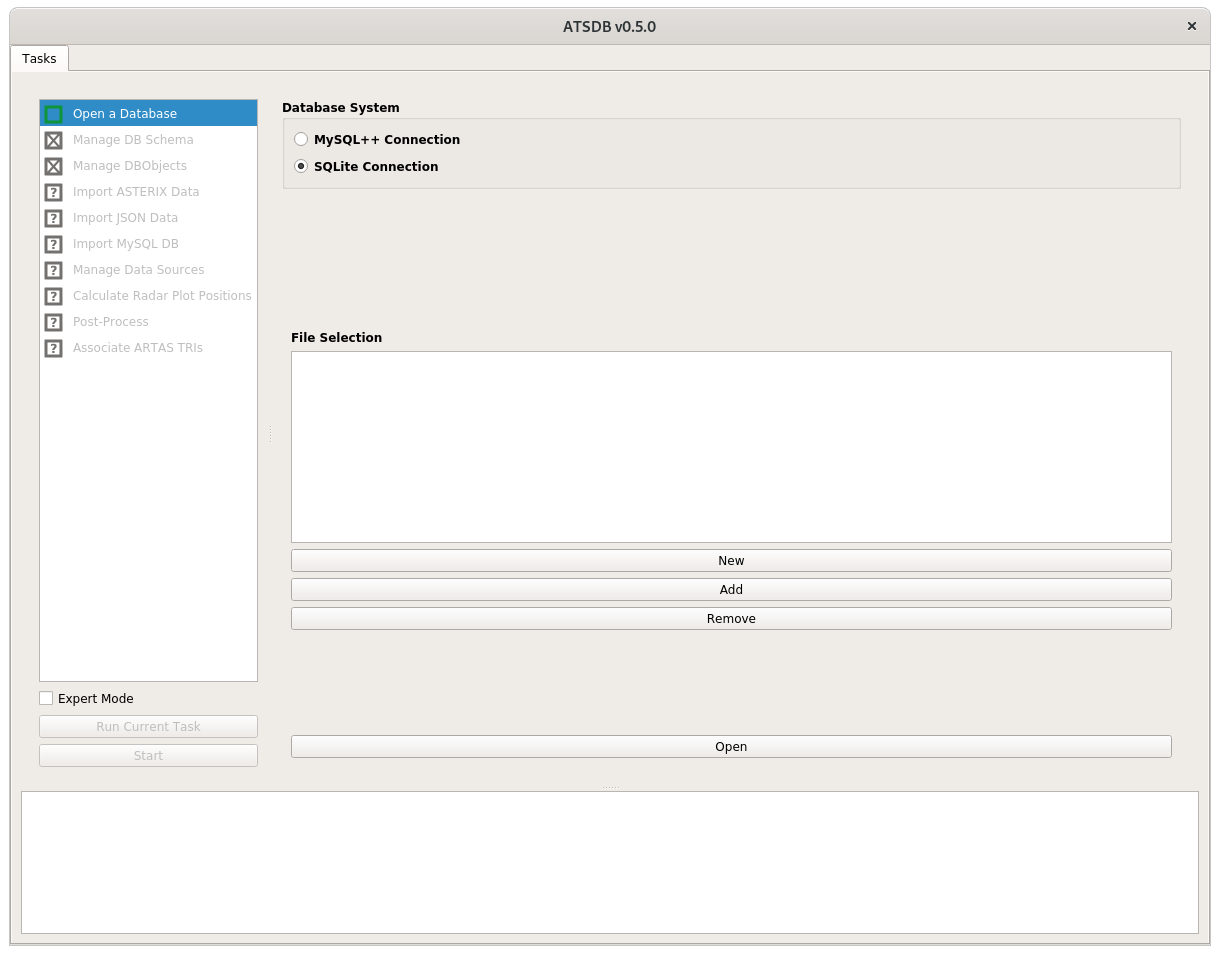
\includegraphics[width=18cm,frame]{../screenshots/db_config_connect.png}
  \caption{Connecting to a database}
  \label{fig:db_connect}
\end{figure}

On the left-hand side, a database system can be selected.  Choices are either MySQL database or a file container with a SQLite3 database. \\
On the lower left (depending on the database system) either a MySQL server connection can be configured or a list of SQLite3 files is shown.\\

On the right-hand side a database schema can be selected and edited (editing is only recommended for experienced users). 
